\documentclass[UTF8,ctexart,a4paper,11pt,openany]{article}
\usepackage[slantfont,boldfont]{xeCJK}
\usepackage{fontspec}
\usepackage{ctex}

\setCJKmainfont{SimSun}%[BoldFont=SimHei] %去掉注释:bf字体为黑体

\setsansfont{SimHei}
\setCJKsansfont{SimHei}

\xeCJKsetcharclass{"2160}{"2470}{1}% 1: CJK
\xeCJKsetup{AutoFallBack=true}
\setCJKfallbackfamilyfont{\CJKrmdefault}{SimSun.ttf}

%\setmainfont{Times New Roman}     %去掉注释:Times new roman字体
%\usepackage{mathptmx}             %去掉注释:Times new roman字体

\usepackage{mathtools}
\usepackage{amsmath}
\usepackage{amsfonts}
\usepackage{amssymb}
\usepackage{amsthm}
\usepackage[T1]{fontenc}
\usepackage{indentfirst} %段首空两格

\usepackage{graphicx}
\usepackage{geometry}
\usepackage{latexsym}
\usepackage{fancyhdr}
\usepackage{epstopdf}
%\usepackage{pifont}
%\usepackage[perpage,symbol*]{footmisc}
\usepackage{titlesec}
\usepackage{setspace}
\usepackage{enumerate}
\usepackage{enumitem}
\usepackage{multicol}
\usepackage{url}
\usepackage{exscale}
\usepackage{ulem}
\usepackage{relsize}
\usepackage{mathrsfs}
\usepackage{tikz}
\usepackage{wrapfig}
\usepackage{framed}
\usepackage{bm}
%\usepackage{pstricks,pst-node,multido,ifthen,calc}
\usepackage[all]{xy}
\usepackage{extarrows}
%\usepackage[backref]{hyperref}
\usepackage{hyperref}
\usepackage{stfloats} %插图的时候不分页

\setlength{\parindent}{2em} %段首空两格
\linespread{1.2}
\usepackage{listings}
\usepackage{xcolor}
\usepackage{algorithm}
\usepackage{algorithmicx}
\usepackage{algpseudocode}
\usepackage{mdframed}
\usepackage{extarrows}
\usepackage{diagbox}
\usepackage{makecell}

\theoremstyle{definition}
\mdfdefinestyle{theoremstyle}{%
linecolor=green!40,linewidth=.5pt,%
backgroundcolor=green!10,
skipabove=8pt,
skipbelow=5pt,
innerleftmargin=7pt,
innerrightmargin=7pt,
frametitlerule=true,%
frametitlerulewidth=.5pt,
frametitlebackgroundcolor=green!35,
frametitleaboveskip=0pt,
frametitlebelowskip=0pt,
innertopmargin=.4\baselineskip,
innerbottommargin=.4\baselineskip,
shadow=true,shadowsize=3pt,shadowcolor=black!20,
%theoremseparator={\hspace{1pt}},
theoremseparator={.},
nobreak=true,
}


\everymath{\displaystyle}

\newtheorem{definition}{\hspace{2em}定义}[section]
\newtheorem{axiom}{\hspace{2em}公理}

\mdtheorem[style=theoremstyle]{theorem}{定理}
\mdtheorem[style=theoremstyle]{example}{例}
\mdtheorem[style=theoremstyle]{exercise}{问题}
\newtheorem{lemma}[theorem]{\hspace{2em}引理}
\newtheorem{corollary}[theorem]{\hspace{2em}推论}

\newcommand*{\QED}{\hfill\ensuremath{\square}}
\newcommand*{\rmk}{\textbf{注:}}
\renewcommand*{\proof}{\textbf{证明:}}
\newcommand*{\tips}{\textbf{提示:}}
\newcommand*{\hard}{\textbf{\color{red}(难)}}
\newcommand*{\eqsmall}{\setlength\abovedisplayskip{1pt}\setlength\belowdisplayskip{1pt}}
\geometry{left=2cm,right=2cm,top=2cm,bottom=2cm}
% \title{数值分析上机报告(示例}
% \author{Fiddie}
\pagestyle{fancy}
\fancyfoot[C]{}
\fancyhead[RO]{ \thepage}
\fancyhead[LE]{\thepage  }
% \fancyhead[RE]{\rightmark (By Fiddie)}
% \fancyhead[LO]{\leftmark (By Fiddie)}
\titleformat{\chapter}{\centering\huge\bfseries}{第\,\thechapter\,章}{1em}{} %更改标题样式
\titleformat{\section}{\bfseries\Large}{$\S$\,\thesection\,}{1em}{} %更改标题样式
\titlespacing*{\chapter}{0pt}{9pt}{0pt} %调整标题间距
\setenumerate[1]{itemsep=0pt,partopsep=0pt,parsep=\parskip,topsep=0pt} %设置enumerate行间距
\setenumerate[2]{itemsep=0pt,partopsep=0pt,parsep=\parskip,topsep=0pt} %设置enumerate行间距
\setitemize[1]{itemsep=0pt,partopsep=0pt,parsep=\parskip,topsep=0pt} % 设置itemize行间距
\setlist[enumerate,2]{label=(\arabic*),topsep=0mm,itemsep=0mm,partopsep=0mm,parsep=\parskip}
    % 设置二层枚举为(1)样式
    
\newfontfamily\hei{SimHei}
\newcommand\textcf[1]{\textbf{\textsf{\hei{#1}}}}

\newcommand\e{\leftarrow}
%\renewcommand{\bibname}{参考文献}

\begin{document}
\begin{center}
{\huge \textbf{数值分析第5次上机作业}}

{\large 学号:221840189,姓名:王晨光}
\end{center}

\section{问题}
    求$f(x)=e^x$在区间$[0,1]$上的$n$次最佳平方逼近多项式(分以下四种情况)$$\varphi (x)=\sum_{k=0}^{n}a_k\varphi_k(x),$$
    \begin{itemize}
        \item $n=5,\varphi_k(x)=x^k;$
        \item $n=5,\varphi_k(x)$为$k$次Legendre多项式;
        \item $n=10,\varphi_k(x)=x^k;$
        \item $n=10,\varphi_k(x)$为$k$次Legendre多项式;
    \end{itemize}
\section{算法思路}
取权函数$W(x)=1$,要求$f(x)=e^x$的$n$次最佳平方逼近多项式,即要求$\varphi^* \in \Phi_n =\mathrm{span}\{ \varphi_0,\varphi_1,\cdots,\varphi_n \}$,使得
\begin{align*}
      \Vert f-\varphi^* \Vert_2^2 &=\int_{a}^{b}[f(x)-\varphi^*(x)]^2 \mathrm{d}x\\
      &=\underset{\varphi \in \Phi_n}{\mathrm{inf} }\int_{a}^{b}[f(x)-\varphi(x)]^2 \mathrm{d}x
\end{align*} 

令$$\varphi(x)=a_0\varphi_0(x)+a_1 \varphi_1(x)+\cdots+a_n \varphi_n(x)$$
$$F(a_0,a_1,\cdots,a_n)=\int_{a}^{b}[f(x)-\sum_{k=0}^n a_k \varphi_k(x)]^2 \mathrm{d}x$$
\\则问题转化为求$F$的极小值
$$
\dfrac{\partial F}{\partial a_j}=2 \int_{a}^{b}[f(x)-\sum_{k=0}^n a_k \varphi_k(x)][-\varphi_j(x)] \mathrm{d}x=0,\;j=0,1,\cdots,n
$$
由此可得
\[
    \sum_{k=0}^n(\varphi_j,\varphi_k)a_k=(f,\varphi_j),\quad j=0,1,\cdots,n
\]
由此,只需储存矩阵$G=((\varphi_j,\varphi_k))_{n+1}$与列向量$f_{ph}=((f,\varphi_0),\cdots,(f,\varphi_n))^T$,令$a=(a_0,a_1,\cdots,a_n)^T$,再解线性方程组$G\cdot a = f_{ph}$即可求出$a_j,j=0,1,\cdots,n$. \\ \indent
当$\varphi_k(x)$为Legendre多项式时,由于\{$\varphi_j(x)\}_{j=0}^n$为直交函数系,$G=((\varphi_j,\varphi_k))_{n+1}$为对角阵,故可直接用向量储存对角线元素.

\begin{algorithm}[H]
    \caption{返回$a$以及逼近函数图像}
    \begin{algorithmic}[1]
        \Require 逼近次数$n$
        \Ensure 系数向量$a$
        \Function {CoefficientAcquisition}{$n$}
            \State 初始化$G$矩阵或向量以及$f_{ph}$向量
            \For {$i$ from 0 to $n$}
                \For {$j$ from 0 to $n$}
                    \State $G_{i,j}\e (\varphi_i, \varphi_j)$
                \EndFor 
                \State $f_{ph}^i \e (f,\varphi_i)$
            \EndFor
            \State $a \e G^{-1}\cdot f_{ph}$
            \State $\varphi \gets \sum_{i=0}^n a_i\varphi_i(x)$
            \State 作出$\varphi $与$f$的函数图像
            \State \Return $a$
        \EndFunction
    \end{algorithmic}
\end{algorithm}
\section{结果分析}%重点(误差图、结果图、分析算法的收敛性(速度)、内存使用(时间、空间)、计算量、稳定性
以下为程序测试结果,返回了图像以及对应的系数$a$。\\ \indent
    1.\;当$n=5$时\\

    \begin{table}[H]
        \centering
        \begin{minipage}{0.49\linewidth}
            \centering
            \begin{tabular}{|c|c|}
            \hline
        $i$& $a_i$\\
    \hline
        0 &  0.9999975939481748\\
        \hline
        1 &  1.000099801486657 \\
        \hline
        2 &  0.49901917513980787 \\
        \hline
        3 &  0.1704895392633275\\
        \hline
        4 &  0.03480111544339166\\
        \hline
        5 &  0.013872004898576736\\
        \hline
            \end{tabular}
            \caption{$n=5,\varphi_i(x)=x^i$系数}
        % \label{table:NormalSafe}
        \end{minipage}
        %\qquad
        \hfill
        \begin{minipage}{0.45\linewidth}
            \centering
            \begin{tabular}{|c|c|}
        \hline
        $i$ &$a_i$  \\
        \hline
        0   &  1.1732975422355196\\
        \hline
        1   &  1.1083386696360753\\
        \hline
        2   &  0.3525658021585433\\
        \hline
        3   &  0.07436115096015425\\
        \hline
        4   &  0.007954540780936126\\
        \hline
        5   &  0.001761524408117519\\
        \hline
            \end{tabular}
            \caption{$n=5,$Legendre多项式系数}
        % \label{table:NormalSafe}
            \end{minipage}
    \end{table}


    \begin{figure}[H]
        \centering
        \begin{minipage}{0.49\linewidth}%表示图片的占用那一列的宽度
            \centering
            %\vspace{-0.6cm}%表示图片与最上方的文字的距离
        %	\setlength{\abovecaptionskip}{0.15cm}%表示caption与图片之间的距离
            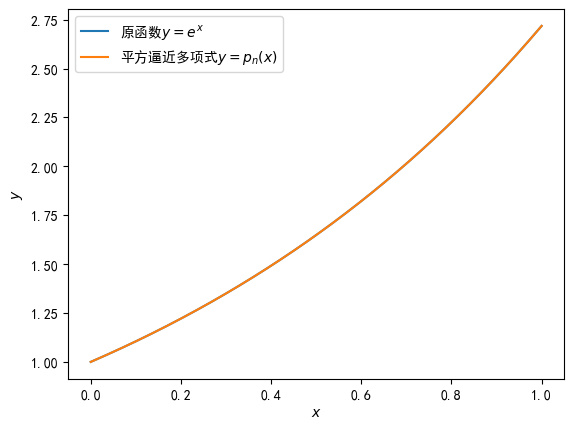
\includegraphics[width=0.9\linewidth]{pics/P5.1.png}
            \caption{$n=5$时 $x^k$逼近}
        \end{minipage}
     \begin{minipage}{0.49\linewidth}
     \centering
     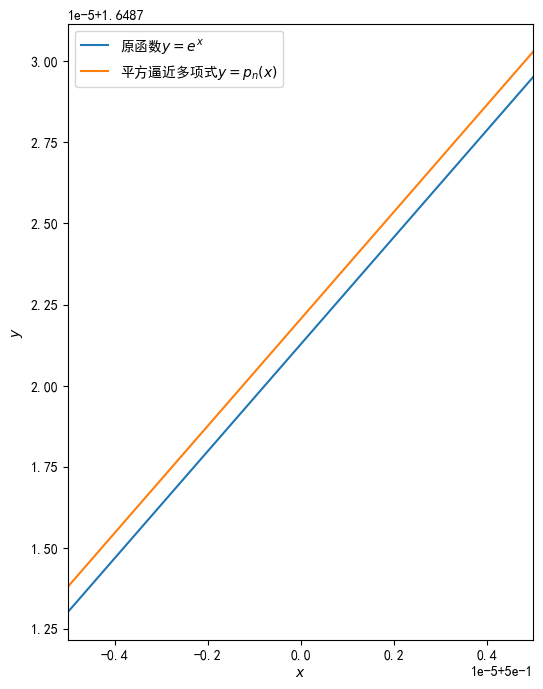
\includegraphics[width=0.9\linewidth]{pics/P5.5.png}
            \caption{$n=5$时 $x^k$逼近(局部)}
        \end{minipage}
    \end{figure}

    \begin{figure}[H]
        %\centering
        %\begin{minipage}{0.49\linewidth}%表示图片的占用那一列的宽度
            \centering
        %%	\setlength{\abovecaptionskip}{0.15cm}%表示caption与图片之间的距离
        
        \begin{minipage}{0.49\linewidth}
            \centering
            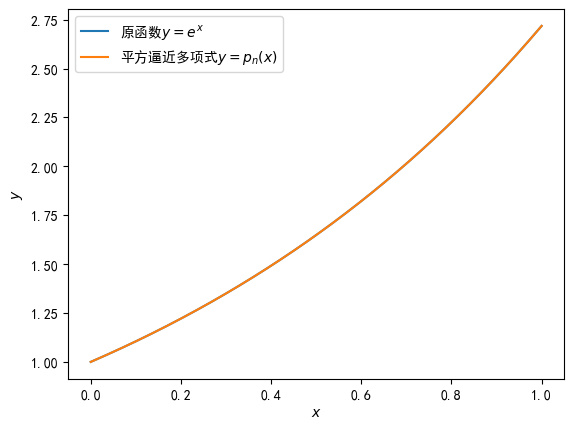
\includegraphics[width=0.9\linewidth]{pics/P5.2.png}
            \caption{$n=5$时 Legendre多项式逼近}
        \end{minipage}
        \begin{minipage}{0.49\linewidth}
            \centering
            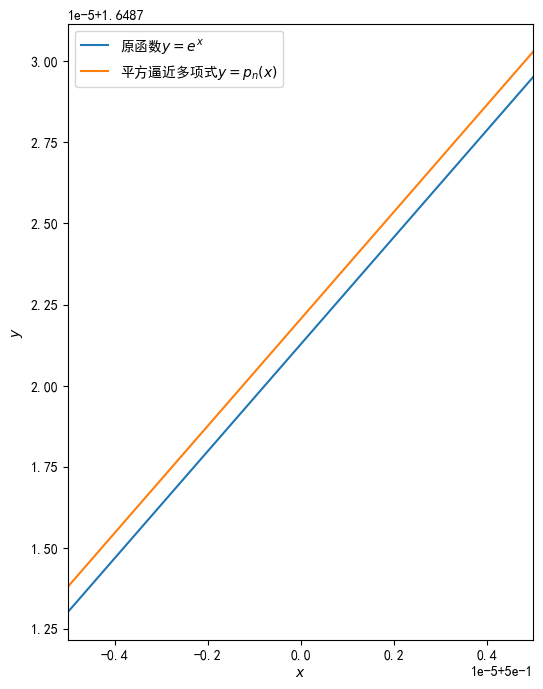
\includegraphics[width=0.9\linewidth]{pics/P5.5.png}
            \caption{$n=5$时 Legendre多项式逼近(局部)}
        \end{minipage}
    \end{figure}
    \newpage
    2.\;当$n=10$时\\

    \begin{table}[H]
        \centering
        \begin{minipage}{0.45\linewidth}
            \centering
            \begin{tabular}{|c|c|}
            
    \hline
            $i$ & $a_i$ \\
            \hline
            0 & 1.0000000012113701 \\
            \hline
            1 & 0.9999998681210073 \\
            \hline
            2& 0.5000035268463334\\
            \hline
            3& 0.16662625984232918 \\
            \hline
            4& 0.04191227935312167\\
            \hline
            5& 0.007455096067967402\\
            \hline
            6& 0.0033287923143171866\\
            \hline
            7& -0.002479244981759852\\
            \hline
            8& 0.0022732391669669206 \\
            \hline
            9& -0.0010475780120787397 \\
            \hline
            10& 0.00020958957362995516\\
            \hline
            \end{tabular}
            \caption{$n=10,\;\varphi_i(x)=x^i$系数}
        % \label{table:NormalSafe}
        \end{minipage}
        %\qquad
        \hfill
        \begin{minipage}{0.45\linewidth}
            \centering
            \begin{tabular}{|c|c|}
        \hline
        $i$ &$a_i$\\
        \hline
        0& 1.17610487769128 \\
        \hline
        1& 1.1012448045699013 \\
        \hline
        2& 0.3609156609890722 \\
        \hline
        3& 0.06749975436161927 \\
        \hline
        4& 0.01221017595693133 \\
        \hline
        5& -0.0002873295948090008\\
        \hline
        6& 0.0007933224883379857 \\
        \hline
        7& -0.0002668997568865246\\
    \hline
        8& 8.219614376558308e-05\\
        \hline
        9& -1.6453268506992322e-05 \\
        \hline
        10& 1.7202942628052338e-06\\
        \hline
            \end{tabular}
            \caption{$n=10,\;$Legendre多项式系数}
        % \label{table:NormalSafe}
            \end{minipage}
    \end{table}

    \begin{figure}[H]
        \centering
        \begin{minipage}{0.49\linewidth}%表示图片的占用那一列的宽度
            \centering
            %\vspace{-0.6cm}%表示图片与最上方的文字的距离
        %	\setlength{\abovecaptionskip}{0.15cm}%表示caption与图片之间的距离
            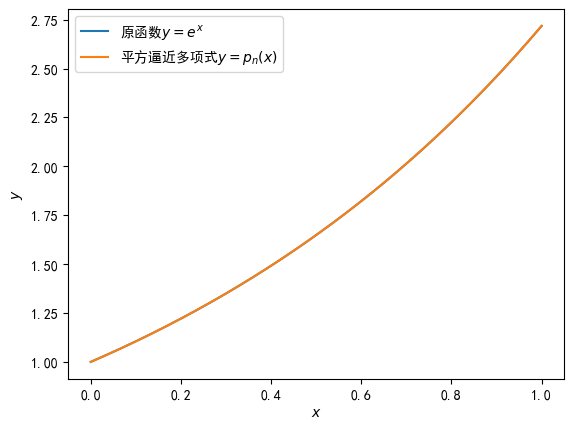
\includegraphics[width=0.9\linewidth]{pics/P5.3.png}
            \caption{$n=10$时 $x^k$逼近}
        \end{minipage}
     \begin{minipage}{0.49\linewidth}
     \centering
     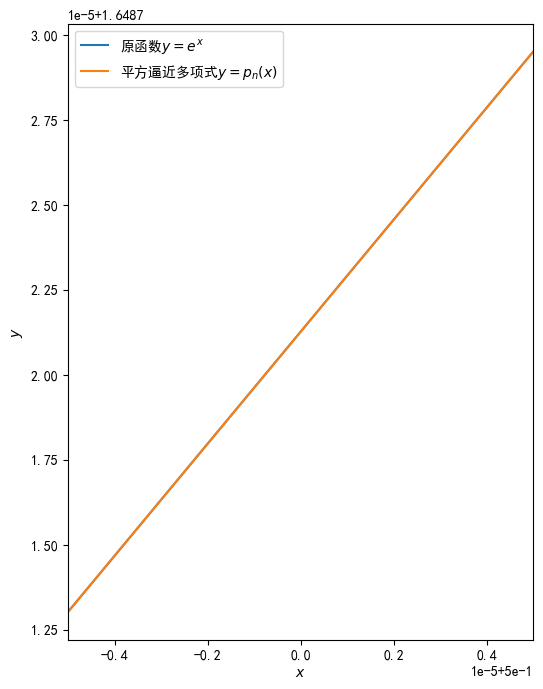
\includegraphics[width=0.9\linewidth]{pics/P5.6.png}
            \caption{$n=10$时 $x^k$逼近(局部)}
        \end{minipage}
    \end{figure}

    \begin{figure}[H]
        %\centering
        %\begin{minipage}{0.49\linewidth}%表示图片的占用那一列的宽度
            \centering
        %%	\setlength{\abovecaptionskip}{0.15cm}%表示caption与图片之间的距离
        
        \begin{minipage}{0.49\linewidth}
            \centering
            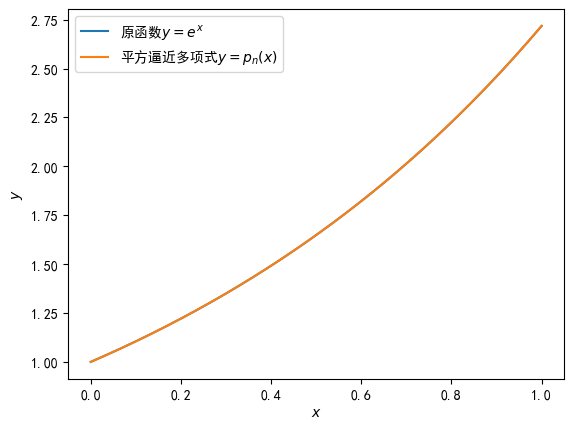
\includegraphics[width=0.9\linewidth]{pics/P5.4.png}
            \caption{$n=10$时 Legendre多项式逼近}
        \end{minipage}
        \begin{minipage}{0.49\linewidth}
            \centering
            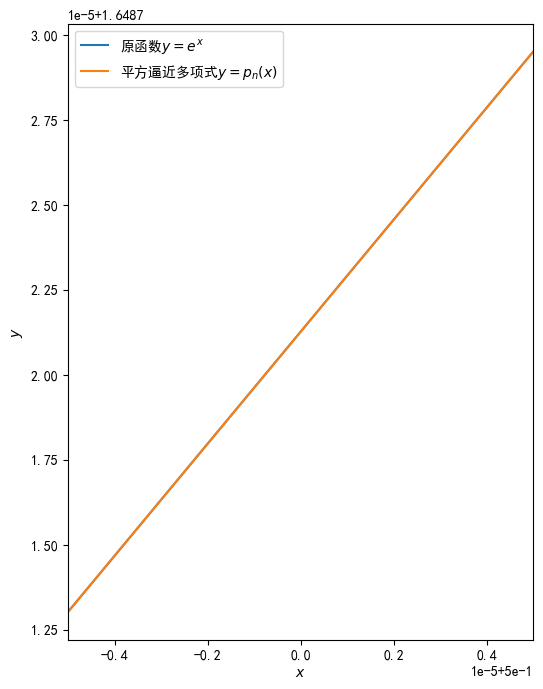
\includegraphics[width=0.9\linewidth]{pics/P5.6.png}
            \caption{$n=10$时 Legendre多项式逼近(局部)}
        \end{minipage}
    \end{figure}
\section{结论}
可以看出,最佳平方逼近可以很好地逼近原函数,且在函数系选取相同的情况下,次数越高,逼近效果越好。
\clearpage

\section{附录: 程序代码}
\lstset{
    numbers=left,
    language=Python,
    keywordstyle=\color{blue!100},
    commentstyle=\color{green!50!blue!50!},
    frame=shadowbox,%阴影
    escapeinside='',%英文分号输入中文
    xleftmargin=2em,xrightmargin=2em,aboveskip=1em,
    framexleftmargin=2em,
    extendedchars=false}

\begin{lstlisting}[aboveskip=0pt]
import numpy as np
import matplotlib.pyplot as plt
from scipy.special import legendre
from scipy.integrate import quad
# display Chinese in gragh
plt.rcParams['font.sans-serif']=['SimHei']
# display "-" in gragh
plt.rcParams['axes.unicode_minus']=False

# 定义原函数
def f(x):
    return np.exp(x)

# 定义正交多项式
def phi(n, k, x, flag):
    if k == 0:
        return np.ones_like(x)
    elif k == 1:
        return x
    elif k > 1:
        if flag == 0:
            return x**k
        elif flag == 1:
            # 使用Legendre多项式
            p = legendre(k)
            return p(x)

# 计算最佳平方逼近多项式系数
def compute_coefficients(n, flag):
    A = np.zeros((n+1, n+1))
    b = np.zeros(n+1)
    for i in range(n+1):
        for j in range(n+1):
            integrand = lambda x: phi(n, i, x, flag) * phi(n, j, x, flag)
            A[i, j], _ = quad(integrand, 0, 1)
        integrand_f = lambda x: f(x) * phi(n, i, x, flag)
        b[i], _ = quad(integrand_f, 0, 1)
    return np.linalg.solve(A, b)

# 生成逼近多项式函数
def approximation_function(n, x, flag):
    coefficients = compute_coefficients(n, flag)
    result = np.zeros_like(x)
    for i in range(n+1):
        result += coefficients[i] * phi(n, i, x, flag)
        print(coefficients[i])
    return result

# 绘制图像
def plot_comparison(n, flag):
    x = np.linspace(0, 1, 1000)
    plt.plot(x, f(x), label='原函数$y=e^x$')
    plt.plot(x, approximation_function(n, x, flag), label='平方逼近多项式$y=p_{n}(x)$')
    plt.xlabel('$x$')
    plt.ylabel('$y$')
    # plt.title('Comparison between original and approximation function (n={})'.format(n))
    plt.legend()
    plt.show()

# 绘制局部放大图像
def plot_local_enlargement(n, flag):
    x = np.linspace(0.499995, 0.500005, 1000)
    plt.figure(figsize=(6, 8))
    plt.plot(x, f(x), label='原函数$y=e^x$')
    plt.plot(x, approximation_function(n, x, flag), label='平方逼近多项式$y=p_{n}(x)$')
    plt.xlabel('$x$')
    plt.ylabel('$y$')
    # plt.title('Comparison between original and approximation function (n={})'.format(n))
    plt.xlim(0.499995, 0.500005)
    plt.legend()
    plt.show()

# plot the gragh and print the coefficients
plot_comparison(5,0)  # n=5, x^k
plot_comparison(5,1)  # n=5, Legendre polynomial
plot_comparison(10,0) # n=10, x^k
plot_comparison(10,1) # n=10, Legendre polynomial
plot_local_enlargement(10, 0)
plot_local_enlargement(5, 0)
\end{lstlisting}

\clearpage

\bibliographystyle{unsrt}
\bibliography{Reference}
\end{document}